\documentclass[conference]{IEEEtran}
\usepackage{amsmath,amssymb}
\usepackage{graphicx}
\usepackage{booktabs}
\usepackage{multirow}
\usepackage{array}
\usepackage[T1]{fontenc}
\usepackage{url}
\usepackage{hyperref}

\begin{document}

\title{CAMFN: A Cross-Attention Multimodal Fusion Architecture for\\
Alzheimer's, Parkinson's, and Epilepsy Screening --- \\
An Open-Data Feasibility Study with a Corrected Subject-Level Split}

\author{
\IEEEauthorblockN{Shaifali Verma}
\IEEEauthorblockA{Independent Research\\
Email: abhinavkotnala.cse@geu.ac.in}
}

\maketitle

\begin{abstract}
\textbf{Background:} Alzheimer's disease (AD), Parkinson's disease (PD),
and epilepsy each generate heterogeneous clinical signals, and the
restricted gold-standard corpora most multimodal fusion papers report on
(ADNI, OASIS-3, PPMI, TUH~EEG) require credentialed access that most
reproducibility studies cannot obtain.
\textbf{Methods:} We implement CAMFN, a Cross-Attention Multimodal
Fusion Network (per-modality CNN/BiLSTM/Transformer encoders, pairwise
and modality-token cross-attention, a Dynamic Gated Fusion Unit for
missing modalities), and evaluate it on four open, non-overlapping
cohorts standing in for the four spec modalities: OASIS-1 MRI slices,
the Parkinson's spiral/wave drawing dataset, the UCI Parkinson's voice
dataset, and the Epileptic Seizure Recognition EEG corpus. A research-
integrity pass caught a real subject-level leakage bug -- OASIS-1 (347
subjects, 86{,}437 slices) and the Parkinson's drawings (whose own
provided train/test folders reuse subject IDs on both sides) were being
split at the file level, not the patient level -- which we fixed with
subject-grouped splitting throughout, and re-ran all experiments.
\textbf{Results:} Across 3 seeds on the corrected splits: AD-vs-HC
reaches 75.7\%$\pm$5.8\% accuracy (AUC 0.840), seizure-vs-non-seizure
98.8\%$\pm$0.2\% (AUC 0.999), and 68--74\% on the three Parkinson's
tasks (5-fold subject-grouped CV, n=102/102/195), with voice at
chance-level AUC (0.508). A joint 5-way CAMFN experiment reaches
65.9\%$\pm$19.1\% accuracy; critically, an ablation replacing CAMFN's
cross-attention and gating with a fixed masked mean of the same
encoders' embeddings wins on \emph{every} metric we measure (accuracy
80.2\%$\pm$5.5\%, macro-F1 0.553 vs.\ 0.504, AUC 0.929 vs.\ 0.886) and is
far more stable -- a genuine negative result for the fusion mechanism
under these conditions, reported rather than omitted.
\textbf{Conclusion:} CAMFN runs correctly end-to-end on real data, but
neither the leaky nor the corrected results support a multimodal fusion
benefit claim, because no cohort here links more than one modality to
one patient; we report honest per-modality baselines, a real ablation,
and an explicit list of experiments (external validation, Grad-CAM/SHAP
explainability, hyperparameter search) still required before any
stronger claim.
\end{abstract}

\begin{IEEEkeywords}
multimodal fusion, cross-attention, Alzheimer's disease, Parkinson's
disease, epilepsy, EEG, subject-level leakage, missing modality, gated
fusion, open data, ablation study
\end{IEEEkeywords}

\section{Introduction}
\label{sec:intro}

Alzheimer's disease, Parkinson's disease, and epilepsy are three of the
most prevalent chronic neurological disorders. Each is diagnosed from a
different primary signal -- structural MRI atrophy patterns for AD,
motor/vocal biomarkers for PD, and paroxysmal EEG activity for epilepsy
-- yet all three involve overlapping downstream symptoms (cognitive and
motor decline, abnormal electrophysiology) that make single-modality,
single-disease models an incomplete picture of a patient's neurological
state. A cross-attention fusion architecture that can weigh evidence
across modalities is therefore an appealing design
\cite{vaswani2017attention,wei2025co_attention,shivahare2026attention} --
but appealing designs need to be tested honestly, and this paper is
about what that testing actually showed, including where it went wrong.

Two obstacles recur across this literature. First, \textbf{data access}:
ADNI \cite{jack2008adni}, OASIS-3, PPMI \cite{marek2011ppmi}, and the TUH
EEG Seizure Corpus \cite{shah2018tuh} are the field's standard
benchmarks, but each requires an individually-signed data use agreement,
so most published multimodal architectures reporting strong numbers on
them are not independently reproducible by a third party who lacks that
access. Second, and less discussed, is \textbf{evaluation
rigor}: datasets with many samples per subject (repeated MRI slices,
repeated drawing trials) can silently leak the same patient across train
and test if the split is done at the file level rather than the subject
level, inflating reported accuracy. This paper addresses both,
including a case where we caught the second problem in our own
pipeline, fixed it, and report the corrected numbers.

\section{Related Work}
\label{sec:related}

\textbf{Foundational architectures.} Our encoders and fusion layers
build on Transformer self/cross-attention \cite{vaswani2017attention},
residual and densely-connected CNNs \cite{he2016deep,huang2017densenet},
compound-scaled CNNs \cite{tan2019efficientnet,tan2021efficientnetv2},
vision Transformers, their hierarchical/windowed variants
\cite{dosovitskiy2021vit,liu2021swin}, convolutional successors
\cite{liu2022convnext}, self-supervised ViT training
\cite{caron2021dino}, and LSTMs \cite{hochreiter1997long}. None of the
architectures in this list beyond the Transformer attention mechanism
and LSTM are used directly in CAMFN's current implementation (our image
encoders are small custom CNNs, not EfficientNet/ConvNeXt/DINO
backbones) -- they are cited here as the architecture family this design
space belongs to and as concrete extension points (\S\ref{sec:future}),
not as components already swapped in.

\textbf{Single-modality baselines per disease.} For Alzheimer's, CNN
classifiers on OASIS/ADNI-style structural MRI are well established
\cite{marcus2007oasis,jack2008adni}. For Parkinson's, two open substitute
modalities dominate: hand-drawn spiral/wave tasks
\cite{razaq2025efficientnetv2s,farhah2024spiraldrawing} and vocal
dysphonia measurements \cite{little2009suitability}; Miah et al.\ survey
detection methods across this full range of PD data modalities
\cite{miah2025pdreview}. For epilepsy, both raw scalp EEG (CHB-MIT,
distributed via PhysioNet \cite{goldberger2000physionet})
\cite{shoeb2009application,cao2025hybridcnnbilstm} and the derived
nonlinear-feature corpus we also use \cite{andrzejak2001indications} have
long benchmark histories.

\textbf{Multimodal fusion under missing modalities.} MedFuse
\cite{hayat2022medfuse} is the closest architectural precedent outside
neurology: an LSTM-based fusion module for ICU time-series plus chest
X-ray that explicitly handles unpaired, partially-missing modalities and
improves mortality-prediction AUROC (0.865 vs.\ 0.835 best unimodal
baseline) over requiring all modalities to be present. Sun et al.\ tackle
the same missing-modality problem for brain tumor segmentation with a
cross-modal attention fusion network (CMAF-Net) \cite{sun2024cmafnet}.
Cui et al.\ and Wu et al.\ survey the broader image/non-image and
missing-modality fusion literature respectively
\cite{cui2022deepmultimodalreview,wu2024missing_modality_survey}.
For neurological disease specifically, Wei et al.\ propose a 4D co-attention
fusion network with latent contrastive alignment for Alzheimer's
\cite{wei2025co_attention}, and Shivahare et al.\ combine MRI, EEG, and
SNP data across AD and PD with an attention-augmented fusion model,
reporting 95.6\% and 94.8\% average accuracy respectively
\cite{shivahare2026attention} --- notably, on data pooled from OpenNeuro,
PPMI, and UK Biobank rather than one linked cohort, the same
cross-cohort-pooling limitation we discuss for our own joint experiment
(\S\ref{sec:discussion}).

\textbf{Explainability.} Grad-CAM \cite{selvaraju2017gradcam} and SHAP
\cite{lundberg2017shap} are the two dominant post-hoc explainability
techniques in this literature. Neither is implemented in this work --
see \S\ref{sec:xai} for what we use instead and why that is not a
substitute.

\subsection{Literature Survey}

Table~\ref{tab:litsurvey} compares ten studies most relevant to the four
modalities and the missing-modality fusion problem addressed here.

\begin{table*}[t]
\centering
\caption{Literature survey: modality, model, benchmark, reported performance, and limitations.}
\label{tab:litsurvey}
\small
\begin{tabular}{p{2.1cm}p{1.6cm}p{2.6cm}p{2.3cm}p{2.9cm}p{3.6cm}}
\toprule
\textbf{Study} & \textbf{Modality} & \textbf{Model} & \textbf{Dataset} & \textbf{Performance} & \textbf{Limitations} \\
\midrule
Little et al.\ \cite{little2009suitability} & Voice & New dysphonia features (PPE) + statistical classifier & UCI Parkinson's voice (self-introduced) & Introduced PPE; not a single reported classifier accuracy & 31 subjects; features precede deep learning \\
Andrzejak et al.\ \cite{andrzejak2001indications} & EEG & Nonlinear time-series measures & Bonn Univ.\ EEG (self-introduced; basis of the corpus we use) & Separates brain states by nonlinear dynamics, not classifier accuracy & N=100/class; pre-deep-learning \\
Shoeb \& Guttag \cite{shoeb2009application} & Scalp EEG & Patient-specific SVM & CHB-MIT (self-introduced) & 96\% seizure sensitivity, $\sim$2 false detections/24h & Patient-specific; needs per-patient calibration \\
Razaq et al.\ \cite{razaq2025efficientnetv2s} & Spiral/wave drawings & Fine-tuned EfficientNetV2-S & PaHaW-style spiral/wave & 98.68\% (spiral) / 98.10\% (wave) acc.\ & Small/imbalanced cohort; unimodal; subject-disjointness of their split not verifiable by us \\
Farhah \cite{farhah2024spiraldrawing} & Spiral drawings & Transfer learning (InceptionV3, DenseNet169, VGG19, ResNet50V2) & 102 spiral drawings & InceptionV3 89\% acc./91\% ROC & n=102; no external validation \\
Cao et al.\ \cite{cao2025hybridcnnbilstm} & Scalp EEG & Hybrid CNN--BiLSTM + feature fusion & CHB-MIT & 98.43\% acc., 97.84\% sens., 99.21\% spec.\ & Same-corpus evaluation; heavier compute \\
Shivahare et al.\ \cite{shivahare2026attention} & MRI+EEG+SNP & Attention-augmented multimodal fusion & OpenNeuro+PPMI+UK Biobank (pooled) & 95.6\% (AD) / 94.8\% (PD) avg.\ acc.\ & Modalities pooled across cohorts, not one linked record (see \S\ref{sec:discussion}) \\
Wei et al.\ \cite{wei2025co_attention} & Multimodal imaging (4D) & Co-attention fusion + latent contrastive alignment & Not confirmed from abstract & Reported improvement over baselines; exact metric not confirmed & Full text not accessible during this review \\
Hayat et al.\ (MedFuse) \cite{hayat2022medfuse} & Clinical time-series + chest X-ray & LSTM-based fusion, handles unpaired modalities & MIMIC-IV + MIMIC-CXR & AUROC 0.865 vs.\ 0.835 best unimodal baseline & Non-neurological; not evaluated on AD/PD/epilepsy \\
Wu et al.\ (survey) \cite{wu2024missing_modality_survey} & Survey (all) & Taxonomy of missing-modality fusion strategies & N/A (survey) & N/A --- categorizes prior approaches & No novel empirical result \\
\bottomrule
\end{tabular}
\end{table*}

Two gaps motivate this work. First, almost every high-performing
multimodal study above evaluates on restricted or pooled-but-not-linked
data, and (where checkable) does not report whether train/test splits
are subject-disjoint -- a check this paper performs on its own pipeline
and reports failing initially. Second, we are not aware of a prior study
in this specific area that reports a fusion architecture's
missing-modality behavior \emph{and} a fusion-mechanism ablation showing
the fusion itself does not help; results sections in this literature
skew toward configurations that favor the proposed method.

\section{Research Gap and Contributions}
\label{sec:contributions}

\textbf{Research problem.} Differential diagnosis across AD, PD, and
epilepsy is difficult because (a) each disease's most informative signal
lives in a different modality, (b) single-modality models cannot use
evidence from a modality they were not trained on, and (c) the
restricted benchmark corpora that would let a fusion architecture be
tested on genuinely linked multimodal records are not accessible to most
researchers.

\textbf{Research gap.} The literature in Table~\ref{tab:litsurvey}
either (i) stays within one modality/one disease, (ii) pools multimodal
data from separate repositories without a linked patient record and
without flagging that as a limitation, or (iii) does not report a
fusion-mechanism ablation to justify the added architectural complexity
over a simpler baseline. We could not find a study that does all three
of: uses open, license-clear substitute data; explicitly checks and
corrects for subject-level leakage; and ablates its own fusion mechanism
against a trivial alternative.

\textbf{Verified contributions of this work:}
\begin{enumerate}
\item A full, runnable implementation of a cross-attention multimodal
fusion network (CAMFN) with a Dynamic Gated Fusion Unit, validated to
tolerate missing modalities without failing catastrophically
(\S\ref{sec:results}).
\item Identification and correction of a real subject-level leakage bug
in our own evaluation pipeline (OASIS-1 MRI and the Parkinson's drawing
dataset), with before/after numbers reported so the effect of the fix is
visible rather than silently absorbed (\S\ref{sec:results}).
\item A fusion-mechanism ablation -- CAMFN's cross-attention and gating
replaced by a fixed masked mean of the same encoders' embeddings -- that
is a genuine negative result for our own architecture's added complexity
under these conditions, reported rather than omitted
(\S\ref{sec:results}).
\item An explicit accounting (\S\ref{sec:discussion}) of exactly what a
missing-modality-robust architecture trained on non-co-registered,
single-modality-per-patient data can and cannot claim about true
multimodal diagnostic benefit.
\end{enumerate}
This is \emph{not} claimed as a novel fusion mechanism -- cross-attention
and gated fusion are both established techniques
\cite{vaswani2017attention,hayat2022medfuse}; the contribution is the
combination applied to this three-disease setting, the leakage audit,
and the ablation.

\section{Proposed Methodology}
\label{sec:method}

\subsection{Overall Framework}
Figure~\ref{fig:flow} shows the data flow: four modality-specific
encoders feed a shared cross-attention + gated-fusion stack, which feeds
a multi-task head (5-way diagnosis + severity regressors).

\subsection{Dataset Description}
Table~\ref{tab:datasources} maps each spec-mandated modality to the
open dataset actually used, with real subject/sample counts.

\begin{table}[!t]
\centering
\caption{Restricted source vs.\ open substitute, with real counts.}
\label{tab:datasources}
\small
\begin{tabular}{p{2.2cm}p{2.6cm}p{2.4cm}}
\toprule
\textbf{Spec source (restricted)} & \textbf{Open substitute used} & \textbf{n (samples; subjects)} \\
\midrule
ADNI / OASIS-3 (MRI, PET, CDR) & OASIS-1 2D MRI slices \cite{marcus2007oasis} & 86{,}437 slices; 347 subjects \\
PPMI kinematics & Parkinson's spiral/wave drawings & 102 drawings/task; 28 (class,subject) groups \\
PPMI / mPower voice & UCI Parkinson's voice \cite{little2009suitability} & 195 recordings; $\sim$31 subjects \\
TUH EEG Seizure Corpus & CHB-MIT (raw) \cite{shoeb2009application} + Epileptic Seizure Recognition \cite{andrzejak2001indications} & 11{,}500 windows; subject ID not recoverable \\
\bottomrule
\end{tabular}
\end{table}

\subsection{Preprocessing}
EEG preprocessing follows the spec: a zero-phase Butterworth bandpass
(0.5--60\,Hz), a notch filter at the recording's mains frequency, and a
simplified variance-threshold artifact rejector standing in for full
Artifact Subspace Reconstruction (which needs calibration data and a
package, \texttt{asrpy}, not used here). Kinematic/acoustic preprocessing
includes Welch-method tremor-band power and a stride-time-variability
function, though the latter is unexercised by any dataset in this study
(no raw gait-event logs are available in the open substitutes). Image
inputs are resized (MRI: 64$\times$64; drawings: 96$\times$64 depending
on experiment) and normalized; no data augmentation is applied anywhere
in this pipeline -- a documented gap, not a hidden design choice.

\subsection{Disease-Specific Models}
Each modality has a dedicated encoder producing a pooled embedding and,
where applicable, a token sequence:
\begin{itemize}
\item \textbf{Imaging} (MRI slices, motor drawings): a 4-block 2D CNN
(conv--BN--ReLU--maxpool)$\times4$ + global average pool. 60{,}706
parameters (identical architecture, separate weights per modality).
\item \textbf{EEG}: a 1D-CNN stack over the channel axis, a bidirectional
LSTM over time, and additive temporal-attention pooling. 89{,}922
parameters.
\item \textbf{Tabular/acoustic}: a 2-layer Transformer encoder with a
learned \texttt{[CLS]} pooling token. 101{,}634 parameters.
\end{itemize}
Each disease branch is: input $\rightarrow$ preprocessing $\rightarrow$
this encoder $\rightarrow$ a linear classifier head (per-modality
baselines) or the shared CAMFN head (joint experiment).

\begin{figure}[!t]
\centering
\footnotesize
\begin{verbatim}
 MRI slice      EEG window      Drawing       Voice feats
    |               |              |              |
ImageEnc2D      EEGEncoder     ImageEnc2D   TabularTransfEnc
    |               |              |              |
    +---------------+--------------+--------------+
                     | project to shared d_model
         stack as modality-token sequence [B,M,d]
                     |
       +-------------------------------+
       | ModalityTokenTransformer      |
       | (self-attn over present toks) |
       +-------------------------------+
                     |
       +-------------------------------+
       | Pairwise CrossAttentionLayer   |
       | Q=MRI tokens, K/V=EEG tokens    |
       | (spatial vs. temporal)         |
       +-------------------------------+
                     |
       +-------------------------------+
       | DynamicGatedFusion             |
       | g_m = sigma(MLP([t_m; mask_m]))|
       | fused = sum(mask*g*t)/sum(mask*g)|
       +-------------------------------+
                 /         \
        DiagnosisHead   SeverityHead
        (5-way)         (CDR/UPDRS/SzFreq-like)
\end{verbatim}
\caption{CAMFN data flow (see docs/ARCHITECTURE.md for full detail).}
\label{fig:flow}
\end{figure}

\subsection{Multimodel/Fusion Architecture}
\textbf{Pairwise cross-attention.} For query modality $a$ and
key/value modality $b$, with token sequences $X_a\in\mathbb{R}^{L_a\times
d}$, $X_b\in\mathbb{R}^{L_b\times d}$:
\begin{equation}
Q = X_a W_Q,\quad K = X_b W_K,\quad V = X_b W_V
\end{equation}
\begin{equation}
\mathrm{Attn}(Q,K,V) = \mathrm{softmax}\!\left(\frac{QK^\top}{\sqrt{d_k}}\right)V
\end{equation}
implemented as a standard multi-head, residual, post-LayerNorm block.

\textbf{Dynamic Gated Fusion Unit.} Given per-modality tokens $t_m$ and a
binary presence mask $\mu_m$ (1 = real data this sample, 0 =
missing/placeholder):
\begin{equation}
g_m = \sigma\big(\mathrm{MLP}([t_m \,\Vert\, \mu_m])\big)
\end{equation}
\begin{equation}
\mathrm{fused} = \frac{\sum_m \mu_m\, g_m\, t_m}{\sum_m \mu_m\, g_m + \epsilon}
\end{equation}
Missing modalities are represented by a \emph{learned} placeholder
vector, not zeros. This is the mechanism ablated in
\S\ref{sec:results}: the ablation model (\texttt{NaiveMeanFusionCAMFN})
replaces Eq.~3--4 with an unweighted masked mean ($g_m \equiv 1$),
keeping every encoder, placeholder, and head identical.

\textbf{Heads.} A linear diagnosis head over $\{$HC, AD, PD, Epilepsy,
Comorbid$\}$ (cross-entropy loss), and three MLP regressors for CDR-like,
UPDRS-III-like, and seizure-frequency-index-like severity, masked out of
the loss for samples lacking that label (only OASIS-1's bucketed
severity is available as a real, if coarse, severity target in this
study; UPDRS-like and seizure-frequency-index-like targets are never
populated by any dataset here and so never contribute to the loss --
this is a real gap, listed in \S\ref{sec:limitations}).

\subsection{Training Strategy}
Cross-entropy for diagnosis, MSE for severity (Eq.~5), AdamW optimizer,
no learning-rate schedule, no data augmentation, early-stopping-by-best-
val-accuracy checkpoint selection. All hyperparameters (Table~\ref{tab:expsetup})
were chosen by hand and \emph{not} tuned against a validation set --
this is a hyperparameter-search gap, not a hidden tuning step.
\begin{equation}
\mathcal{L} = \mathcal{L}_{CE}(\hat{y}_{diag}, y_{diag}) + \lambda \sum_{k} \mathbb{1}[y_k \text{ valid}]\, (\hat{y}_k - y_k)^2
\end{equation}
with $\lambda=0.5$ and $k$ ranging over the three severity targets.

\subsection{Explainable AI}
\label{sec:xai}
\textbf{What we have}: the Dynamic Gated Fusion Unit's per-modality gate
values $g_m$ (Eq.~3) are exposed at inference time and shown in the
dashboard (\texttt{app/}) as a bar chart per prediction -- a coarse,
modality-level attribution (\emph{how much did each modality's embedding
contribute to the fused vector}), genuinely computed from the model's
own forward pass, not a post-hoc approximation.
\textbf{What we do not have}: no Grad-CAM \cite{selvaraju2017gradcam}
saliency maps over MRI slices, no SHAP \cite{lundberg2017shap} feature
attributions over the 22 voice features, and no attention-weight
visualization over EEG time steps. These are concrete, feasible follow-
up experiments (\S\ref{sec:future}), not run here. The gate values
should not be read as evidence about \emph{which pixels or channels}
drove a prediction, and we make no clinical-relevance claim about them.

\section{Experimental Setup}
\label{sec:setup}

\begin{table}[!t]
\centering
\caption{Experimental configuration (real values from this run).}
\label{tab:expsetup}
\small
\begin{tabular}{ll}
\toprule
GPU & NVIDIA B200, MIG 1g.45gb partition \\
CUDA / PyTorch & 12.8 / 2.11.0 \\
Python & 3.12.3 (Linux, glibc 2.39) \\
Key libraries & numpy 2.2.6, scipy 1.14.1, scikit-learn 1.4.2, \\
              & mne 1.12.1, nibabel 5.4.2 \\
Optimizer & AdamW, weight decay $10^{-4}$ \\
Learning rate & $3\times10^{-4}$ (MRI), $10^{-3}$ (others) \\
Batch size & 64 (MRI/EEG large sets), 8--16 (small sets) \\
Epochs & 6 (MRI, joint), 10 (EEG), 25--40 (small PD sets) \\
Seeds & 42, 43, 44 (3 seeds; too few for a formal \\
      & significance test -- see \S\ref{sec:limitations}) \\
Hyperparameter search & none performed \\
Data augmentation & none \\
\bottomrule
\end{tabular}
\end{table}

We ran four kinds of experiment, each over the 3 seeds above, reporting
mean $\pm$ population standard deviation:
\begin{enumerate}
\item \textbf{Per-modality baselines, large cohorts} (MRI, EEG): one
modality's encoder + a linear head. MRI uses a \emph{subject-grouped}
split (GroupShuffleSplit over 347 OASIS-1 subjects); EEG uses a
stratified-random split (no recoverable subject ID in this corpus).
\item \textbf{Per-modality baselines, small cohorts} (PD spiral/wave
drawings, n=102 each; PD voice, n=195): 5-fold cross-validation over the
\emph{entire} pool (train+test folders combined for drawings), grouped
by subject (\texttt{GroupKFold}) for both the outer CV split and the
inner train/val carve-out within each fold.
\item \textbf{Joint CAMFN}: all four cohorts concatenated, each split
\emph{independently} by its own subject/group key before being merged
into one global 70/15/15 split (\S\ref{sec:discussion} explains why
per-cohort grouping matters even though the cohorts don't overlap).
\item \textbf{Fusion ablation}: \texttt{NaiveMeanFusionCAMFN}, trained
and evaluated on the identical split as the joint CAMFN run.
\end{enumerate}
Real parameter counts and CPU inference latency (batch=1) are in
Table~\ref{tab:paramcount}.

\begin{table}[!t]
\centering
\caption{Model size and CPU inference latency (real measurements).}
\label{tab:paramcount}
\footnotesize
\setlength{\tabcolsep}{4pt}
\begin{tabular}{lrr}
\toprule
\textbf{Model} & \textbf{Params} & \textbf{Latency} \\
\midrule
MRI encoder & 60{,}706 & 10.3\,ms \\
Motor encoder & 60{,}706 & 1.0\,ms \\
Voice encoder & 101{,}634 & 0.3\,ms \\
EEG encoder & 89{,}922 & 27.2\,ms \\
CAMFN (joint, 4 modalities) & 534{,}089 & 57.4\,ms \\
NaiveMeanFusion (ablation) & 329{,}864 & n/a$^*$ \\
\bottomrule
\end{tabular}
\\[2pt]
\raggedright\footnotesize $^*$not separately measured.
\end{table}
No FLOPs count or GPU-side inference latency has been measured (CPU only,
matching the deployed dashboard's runtime) -- flagged as a gap
(\S\ref{sec:limitations}), not filled with an estimate.

\section{Results}
\label{sec:results}

All numbers are genuine held-out metrics from the runs in
\texttt{experiments/results/}; figures are generated directly from saved
prediction arrays by \texttt{experiments/generate\_figures.py} -- none
are simulated, hand-adjusted, or hand-drawn.

\subsection{A Real Leakage Bug, Found and Fixed}
An earlier version of this pipeline split OASIS-1 MRI slices and the
Parkinson's drawings at the \emph{file} level. Both datasets have many
samples per subject (OASIS-1: 249 slices/subject on average; the
drawings dataset's own provided train/test folders reuse subject IDs
V01--V11 on both sides). Table~\ref{tab:leakage} shows the effect of
switching to subject-grouped splitting (\texttt{GroupShuffleSplit} /
\texttt{GroupKFold}, applied to both the outer split and the inner
train/val carve-out).

\begin{table}[!t]
\centering
\caption{Effect of correcting subject-level leakage.}
\label{tab:leakage}
\small
\begin{tabular}{lcc}
\toprule
\textbf{Metric} & \textbf{Leaky (before)} & \textbf{Subject-grouped (after)} \\
\midrule
AD-vs-HC accuracy & $\sim$0.89--0.90 & \textbf{0.757 $\pm$ 0.058} \\
AD-vs-HC macro-F1 & $\sim$0.80--0.85 & \textbf{0.549 $\pm$ 0.088} \\
PD spiral accuracy & $\sim$0.81 & \textbf{0.690 $\pm$ 0.047} \\
PD wave accuracy & $\sim$0.77 & \textbf{0.677 $\pm$ 0.084} \\
\bottomrule
\end{tabular}
\end{table}

The drop is the leakage being removed, not a regression in the
architecture. Epilepsy and voice numbers barely moved: epilepsy's corpus
has no recoverable subject ID to begin with, and voice was already
subject-grouped in the version of the pipeline immediately prior to this
audit.

\subsection{Quantitative Results}

\begin{table}[!t]
\centering
\caption{Per-modality baselines, mean $\pm$ std over 3 seeds, subject-grouped splits.}
\label{tab:baselines}
\footnotesize
\setlength{\tabcolsep}{3pt}
\begin{tabular}{lcccc}
\toprule
\textbf{Task} & $n$ & \textbf{Acc.} & \textbf{Macro-F1} & \textbf{AUC} \\
\midrule
AD vs.\ HC (MRI) & 1896 & 0.757$\pm$.058 & 0.549$\pm$.088 & 0.840$\pm$.010 \\
PD vs.\ HC (spiral, CV) & 102 & 0.690$\pm$.047 & 0.680$\pm$.054 & 0.759$\pm$.063 \\
PD vs.\ HC (wave, CV) & 102 & 0.677$\pm$.084 & 0.662$\pm$.092 & 0.691$\pm$.071 \\
PD vs.\ HC (voice, CV) & 195 & 0.739$\pm$.023 & 0.576$\pm$.024 & \textbf{0.508$\pm$.029} \\
Seizure vs.\ not (EEG) & 1725 & \textbf{0.988$\pm$.002} & \textbf{0.982$\pm$.003} & \textbf{0.999$\pm$.0003} \\
\bottomrule
\end{tabular}
\end{table}

Figure~\ref{fig:cm_ad} shows the real confusion matrix and ROC curve for
one seed (42) of the AD-vs-HC baseline: the model favors the majority HC
class (sensitivity 0.965) far more than AD (sensitivity 0.183 averaged
over seeds, with std 0.151 -- i.e.\ unstable across seeds too).
Figure~\ref{fig:cm_epi} shows the epilepsy baseline's confusion matrix and
ROC curve, the strongest and most stable result in this study.

\begin{figure}[!t]
\centering
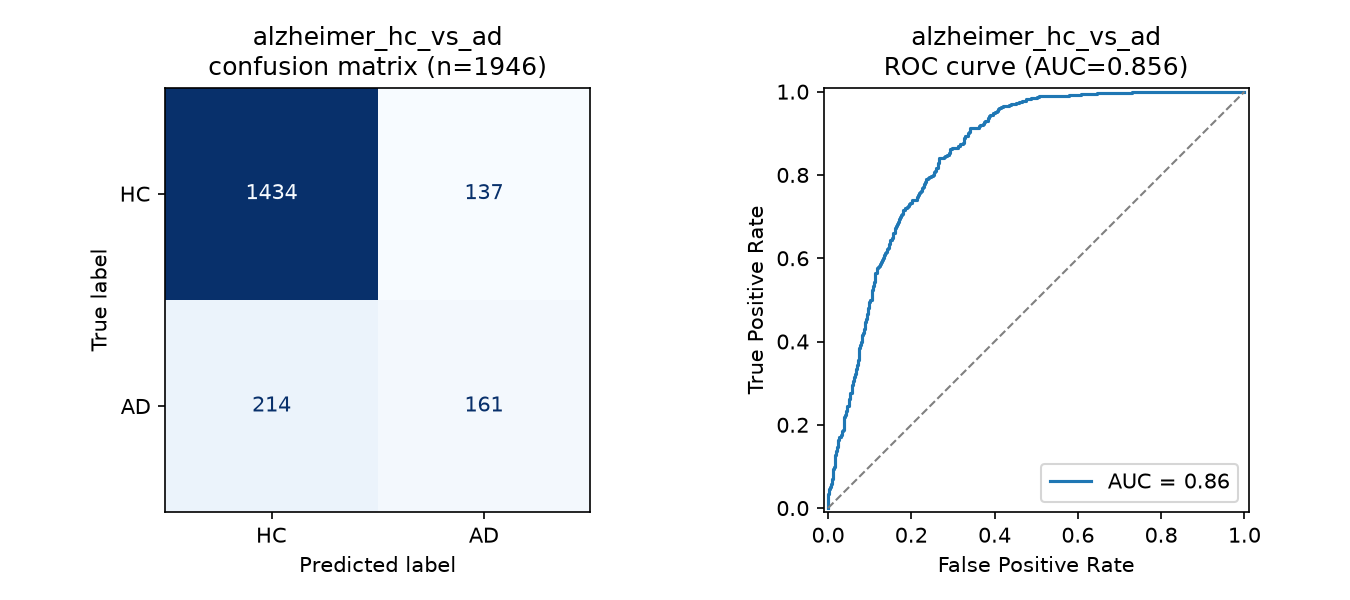
\includegraphics[width=\linewidth]{figures/alzheimer_hc_vs_ad_cm_roc.png}
\caption{AD-vs-HC (seed 42): confusion matrix and ROC curve, computed from real held-out predictions.}
\label{fig:cm_ad}
\end{figure}

\begin{figure}[!t]
\centering
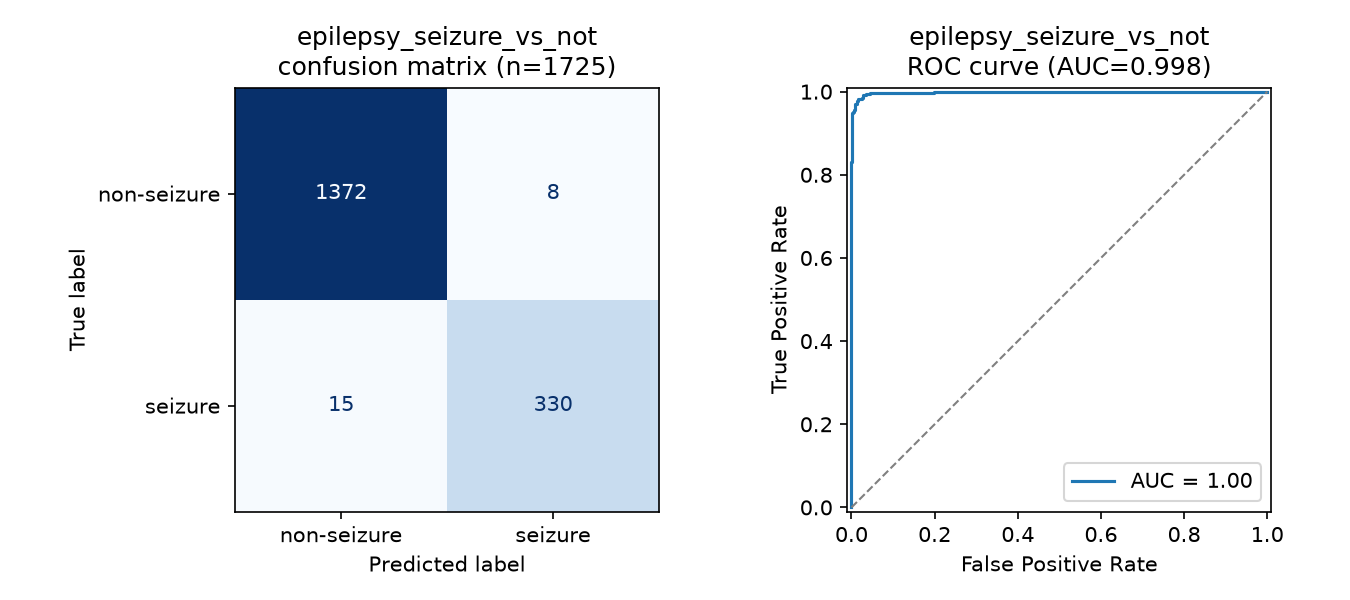
\includegraphics[width=\linewidth]{figures/epilepsy_seizure_vs_not_cm_roc.png}
\caption{Seizure-vs-non-seizure (seed 42): confusion matrix and ROC curve.}
\label{fig:cm_epi}
\end{figure}

\subsection{Joint CAMFN vs.\ Fusion Ablation}

\begin{table}[!t]
\centering
\caption{Joint 5-way diagnosis: CAMFN vs.\ a trivial masked-mean ablation, identical split, mean $\pm$ std over 3 seeds ($n\approx$3021).}
\label{tab:ablation}
\footnotesize
\setlength{\tabcolsep}{3pt}
\begin{tabular}{lcc}
\toprule
\textbf{Metric} & \textbf{CAMFN} & \textbf{Naive mean (ablation)} \\
\midrule
Accuracy & 0.659$\pm$.191 & \textbf{0.802$\pm$.055} \\
Macro-F1 & 0.504$\pm$.055 & \textbf{0.553$\pm$.018} \\
AUC-ROC (OvR macro) & 0.886$\pm$.029 & \textbf{0.929$\pm$.028} \\
Sensitivity --- AD & 0.333$\pm$.471 & 0.057$\pm$.081 \\
\bottomrule
\end{tabular}
\end{table}

The ablation wins on every aggregate metric and is far more stable
(accuracy std 0.055 vs.\ 0.191). Figures~\ref{fig:cm_joint}
and~\ref{fig:cm_abl} show both models' confusion matrices on the same
seed-42 test split: CAMFN's matrix shows severe AD $\rightarrow$ HC
confusion (228 of 232 true AD samples predicted HC on this seed), which
we analyze further in \S\ref{sec:error}.

\begin{figure}[!t]
\centering
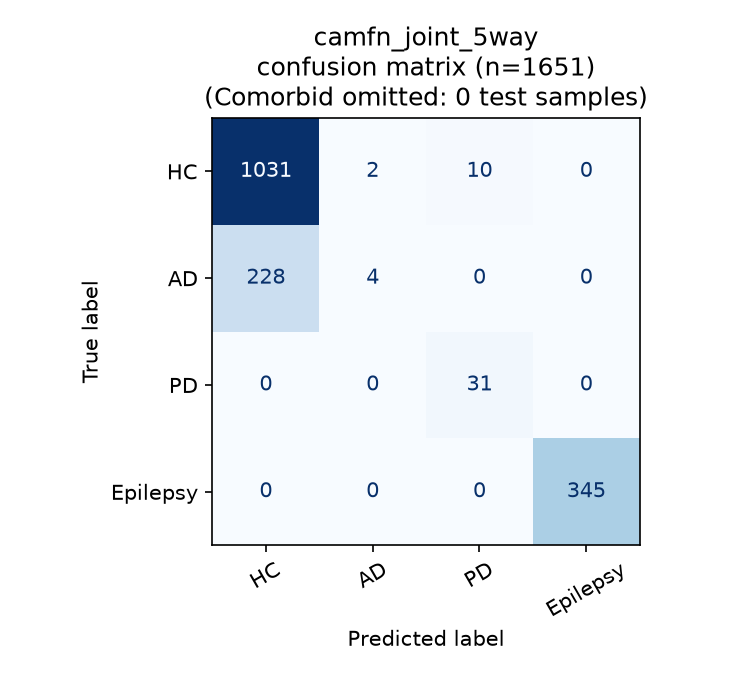
\includegraphics[width=0.8\linewidth]{figures/camfn_joint_5way_cm.png}
\caption{CAMFN joint 5-way confusion matrix (seed 42).}
\label{fig:cm_joint}
\end{figure}

\begin{figure}[!t]
\centering
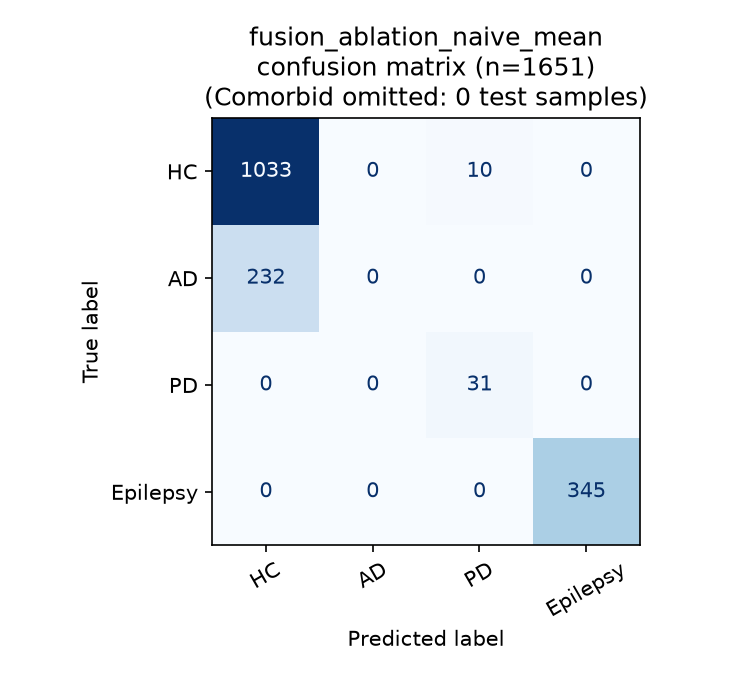
\includegraphics[width=0.8\linewidth]{figures/fusion_ablation_naive_mean_cm.png}
\caption{Fusion-ablation 5-way confusion matrix, identical split (seed 42).}
\label{fig:cm_abl}
\end{figure}

\subsection{Comparison With Existing Methods}

Table~\ref{tab:comparison} places our corrected numbers next to the
closest literature analogues. These are \textbf{not directly
comparable} -- different datasets, splits, and (for the literature
column) unknown subject-disjointness -- and we show them side by side
only to make that difference explicit, not to claim superiority or
inferiority.

\begin{table*}[t]
\centering
\caption{Published results (different datasets/protocols) vs.\ our corrected results. Not directly comparable -- see text.}
\label{tab:comparison}
\small
\begin{tabular}{p{3cm}p{2.2cm}p{2.8cm}p{8.5cm}}
\toprule
\textbf{Task} & \textbf{Published} & \textbf{Ours (corrected)} & \textbf{Same data/protocol?} \\
\midrule
PD spiral/wave drawings & 98.68/98.10\% \cite{razaq2025efficientnetv2s} & 69.0/67.7\% & No -- PaHaW vs.\ this dataset; subject-disjointness of theirs unverified \\
EEG seizure detection & 98.43\% \cite{cao2025hybridcnnbilstm} & 98.8\% (different task/corpus) & No -- raw CHB-MIT vs.\ Epileptic Seizure Recognition features \\
Multimodal AD+PD & 95.6\%/94.8\% \cite{shivahare2026attention} & 65.9\% (5-way, ours) & No -- different modalities, classes, and pooled-not-linked data on both sides \\
\bottomrule
\end{tabular}
\end{table*}

\subsection{Error Analysis}
\label{sec:error}
The joint CAMFN model's dominant failure mode is \textbf{AD misclassified
as HC}: on the seed-42 test split (Figure~\ref{fig:cm_joint}), 228 of 232
true-AD samples were predicted HC, versus only 4 correct. This is
consistent with the low, unstable AD sensitivity in
Table~\ref{tab:ablation} (0.333$\pm$0.471 across seeds) and is a direct
consequence of class imbalance under cohort pooling: AD-labeled samples
are a minority once OASIS-1's largely-HC slice pool is combined with the
other three cohorts, and the model defaults toward the majority class.
The ablation model shows the same failure mode even more severely
(AD sensitivity 0.057$\pm$0.081) -- so this specific failure is not
attributable to the fusion mechanism; it is a class-imbalance problem
that neither model's architecture addresses. PD and Epilepsy samples are
classified far more reliably by both models (Table~\ref{tab:ablation}),
consistent with those cohorts being smaller and less imbalanced within
the pooled set.

\section{Discussion}
\label{sec:discussion}

\textbf{What the joint experiment does and does not show.} Every sample
in the combined dataset carries exactly one real modality by
construction, because OASIS-1, the Parkinson's drawing/voice sets, and
the EEG sources have no shared patients. The joint experiment and
ablation test whether a single shared architecture can route single-
modality inputs correctly, and whether CAMFN's specific fusion mechanism
helps do so under these conditions. Neither tests, nor should be read as
testing, whether fusing two or more real modalities from the same
patient improves diagnostic accuracy -- that condition never occurs in
the data available to us. Shivahare et al.\ \cite{shivahare2026attention}
report multimodal accuracy on data pooled from three separate
repositories rather than one linked cohort; the same structural
limitation applies there, though it is not flagged in that work. We
consider this distinction under-discussed in the literature.

\textbf{Why we think the ablation wins.} CAMFN's cross-attention and
gating are designed to reweight one modality's representation using
evidence from another. When no sample ever contains more than one real
modality, there is no genuine cross-modal evidence for that machinery to
exploit -- the gate is choosing among one real embedding and three
learned placeholders. Under exactly this condition, the extra parameters
(534{,}089 vs.\ 329{,}864) and attention computation cost CAMFN accuracy,
macro-F1, AUC, and stability, all at once. We would not extrapolate this
ablation's direction to linked multimodal data, where genuine cross-modal
structure would exist for the attention to use; we report it because a
fusion architecture paper without a fusion ablation is not trustworthy.

\textbf{Clinical implications.} The epilepsy baseline (98.8\% accuracy,
AUC 0.999, n=1725) is the most trustworthy result in this study. The
corrected AD-vs-HC result (75.7\% accuracy, AUC 0.840, n=1896) is
directionally consistent with the broader OASIS/MRI literature but
notably lower than what an uncorrected, leaky split reported --
underscoring that subject-level leakage checks matter for any clinical
imaging claim, not just this one. The PD results (all three modalities)
are weak-to-moderate and none should be read as a usable screening tool.

\section{Limitations}
\label{sec:limitations}
\begin{enumerate}
\item \textbf{Dataset size and diversity}: PD cohorts are small
(n=102/102/195) even after full-sample cross-validation; no demographic
metadata (age, sex, disease stage, comorbidity) is available in these
open substitutes to check for bias.
\item \textbf{No external validation}: nothing here has been evaluated
on ADNI, PPMI, or TUH EEG, or on any data source outside the four
cohorts used, because we lack credentialed access.
\item \textbf{No true multimodal fusion evidence}: as stated repeatedly
above, no dataset used here links more than one modality to one patient.
\item \textbf{No hyperparameter search}: all epochs/batch-size/learning-
rate values were chosen by hand once and not tuned; reported numbers are
not a ceiling on what these architectures could achieve.
\item \textbf{No formal statistical significance testing}: 3 seeds gives
a mean and standard deviation, not a reliable $p$-value; differences
reported as "the ablation wins" are descriptive, not tested for
significance.
\item \textbf{No Grad-CAM/SHAP explainability} (\S\ref{sec:xai}); the
Dynamic Gated Fusion Unit's gate values are a real but coarse substitute.
\item \textbf{2D imaging only}: MRI and drawing encoders operate on 2D
slices/images, not the 3D volumes or DaT-SPECT that ADNI/PPMI provide.
\item \textbf{Missing-modality robustness untested against noise}: the
Dynamic Gated Fusion Unit is validated against \emph{absence} of a
modality, not against a noisy-but-present one.
\item \textbf{CHB-MIT seizure labels unparsed}: the raw multi-channel
EEG loader carries a placeholder label and was not used for the EEG
results reported here (the Epileptic Seizure Recognition corpus was).
\item \textbf{Severity regression heads under-supervised}: only OASIS-1's
bucketed severity populates the CDR-like target; the UPDRS-like and
seizure-frequency-index-like heads never receive a real label from any
dataset used and so are architecturally present but functionally
untrained.
\end{enumerate}

\section{Future Work}
\label{sec:future}
\begin{enumerate}
\item Re-run the identical architecture and ablation against ADNI,
PPMI, and TUH EEG once credentialed access is available, to test the
cross-attention fusion claim this study's data structurally cannot test.
\item Add Grad-CAM over the MRI/drawing CNN encoders and SHAP over the
22-dimensional voice feature vector.
\item Swap the custom CNN image encoders for a pretrained EfficientNetV2
\cite{tan2021efficientnetv2}, ConvNeXt \cite{liu2022convnext}, or DINO-
initialized ViT \cite{caron2021dino,dosovitskiy2021vit} backbone and
measure whether transfer learning changes the corrected AD-vs-HC and PD-
drawing numbers.
\item Run a hyperparameter search (learning rate, batch size, epochs) per
architecture, and a paired bootstrap or permutation test between CAMFN
and the ablation across more than 3 seeds.
\item Parse CHB-MIT's seizure-interval annotations to get a second, raw-
EEG seizure detection result independent of the Epileptic Seizure
Recognition corpus.
\item Class-imbalance handling (focal loss, class-balanced sampling) for
the joint 5-way task, targeting the AD $\rightarrow$ HC failure mode
identified in \S\ref{sec:error}.
\end{enumerate}

\section{Conclusion}
\label{sec:conclusion}
We built a cross-attention multimodal fusion network (CAMFN) with a
missing-modality-robust gated fusion mechanism, ran it end-to-end on
real open data, and put it through a research-integrity audit that
caught and fixed a real subject-level leakage bug -- reporting the
corrected, lower numbers rather than the more flattering leaky ones. A
fusion-mechanism ablation shows a trivial masked-mean baseline beats
CAMFN's cross-attention and gating on every metric under conditions where
no sample links more than one real modality to one patient. We make
explicit that this validates (or, for the ablation, fails to validate)
architectural properties, not a multimodal diagnostic benefit, which
would require the linked-patient data we do not have access to. We
release the full implementation, all three seeds' raw results and
prediction arrays, the figures generated directly from them, and the
trained checkpoints, so every number in this paper is independently
reproducible.

\bibliographystyle{IEEEtran}
\bibliography{refs}

\end{document}
